\subsection{Stochastic Differential Equations}
\subsubsection{The Itô integral and - process}
A stochastic differential equation (SDE) is a differential equation where at least one term is a stochastic process. We only consider processes driven by a Brownian motion - also known as a Wiener process. To define stochastic differential equations with more rigor we need to define a brownian motion: A brownian motion is a continuous stochastic processes, $W_t\in\mathbb{R}$ where
\begin{enumerate}
    \item $X_0 = 0$ almost surely
    \item $\Delta W_n = W\left(t_{n + 1}\right) - W\left(t_{n}\right)\sim\mathcal{N}\left(0, t_{n + 1} - t_{n}\right)$
    \item $X_{t_1}\indep \left(X_{t_2} - X_{t_1}\right)\indep \dots \indep \left(X_{t_n} - X_{t_{n - 1}}\right), \: 0 < t_1 < t_2 < \dots < t_n$.
\end{enumerate}
Then to define integration from $t_0$ to $t$ of some function $\sigma(X_t, t)$ with respect to $W_t$, we partition the interval $[t_0, t]$ into smaller intervals $[t_k, t_{k + 1}]$ with $t_0 \leq t_1 \leq \dots \leq t_n = t$. The integral is constructed by having the partition get increasingly finer
\begin{align}
    \int_{t_0}^t \sigma^2(X_s, s) \mathrm{d}W_s = \lim_{n \to \infty}\sum_k \sigma\left(X_{t_k}, t_k\right)\left(W_{t_{k + 1}} - W_{t_k}\right),
\end{align}
where the limit is in $L_2$-sense \cite[equation 4.6]{Srkk2019}. We call this the Itô integral and it is an important part of Itô calculus; an area that expands the techniques of calculus to stochastic processes. This relates to stochastic differential equations via the Itô integral equation
\begin{align}
    X_t - x_0 = \int_{t_0}^t b(X_s, s)\mathrm{d}s + \int_{t_0}^t \sigma(X_s, s)\mathrm{d}W_s. \label{eq:itoIntegralEquation}
\end{align}
Note that the first integral on the right hand side merely is a Riemann integral. A stochastic differential equation can then by understood by letting the limits of integration in (\ref{eq:itoIntegralEquation}) be $t$ and $t+\mathrm{d}t$ for some small $\mathrm{d}t$. As shorthand for (\ref{eq:itoIntegralEquation}) we write
\begin{align}
    \mathrm{d}X_t = b(X_t, t)\mathrm{d}t + \sigma(X_t, t)\mathrm{d}W_t, \quad X_{t_0} = x_0 \label{eq:firstSDE},
\end{align}
and this is the general form of an SDE. \\
To better understand stochastic differential equations we need to introduce a bit more nomenclature: The solution, $X_t$, is called an Itô process, and the values it can take is its state space. We refer to the functions $b(X_t, t)$ and $\sigma(X_t, t)$ as the drift- and diffusion coefficients respectively. For ease of language we sometimes leave out the "coefficient" part. In our applications the drift and diffusion depend on some parameter vector, $\theta\in\mathbb{R}^p$ or some subset thereof. For typographical reasons though, we mostly suppress this dependence in the notation. Additionally, we say that term with the diffusion coefficient is the noise term or stochastic term and the term with the drift is the deterministic term or deterministic part. We say that the noise is additive, if the function $\sigma(X_t, t)$ is constant and multiplicative otherwise. Lastly, the stochastic differential equation has autonomous drift or diffusion, when they do not directly depend on time; the system as a whole is autonomous, if both parts are autonomous.\\
Although, the representation in (\ref{eq:firstSDE}) is the most common in the litterature and the one we use for the most part, we have to note that is merely a representation of (\ref{eq:itoIntegralEquation}). If one formally divides by $\mathrm{d}t$ though, we end up with a term, where we take the derivative of the Wiener process. Even though this process has almost surely continuous sample paths, they are nowhere differentiable \cite[theorem 11.22 and theorem 11.35]{Hansen2022}.\\
Now, to motivate the arguably most important result in the study of stochastic differential equations, we consider integrating the Wiener process with respect to itself
\begin{align}
    \int_0^t W_s \mathrm{d}W_s & = \lim_{n \to \infty}\sum_k W_{t_k}\left(W(t_{k + 1}) - W_{t_k}\right) \nonumber \\ 
    & = - \frac{1}{2}\lim_{n \to \infty}\sum_k \left(W(t_{k + 1}) - W(t_{k})\right)^2  + \frac{1}{2}\lim_{n \to \infty}\sum_k\left(W(t_{k + 1})^2 - W(t_{k})^2\right) \nonumber \\
    & = -\frac{t}{2} + \frac{W_t^2}{2}.
\end{align}
We have used the observation that the last sum was telescopic and equal to $W_t^2$. The first sum is the quadratic variation of the wiener process, which by \cite[theorem 11.34]{Hansen2022} is $t$. Put differently
\begin{align}
    \mathrm{d}\left(\frac{1}{2}W_t^2\right) = W_t\mathrm{d}W_t + \frac{1}{2}\mathrm{d}t,
\end{align}
which is not what we would expect from the normal chain rule, ergo Itô calculus needs its own version of the chain rule: Itô's formula \cite[Theorem 4.2]{Srkk2019}.  Given an Itô process, $X_t$, described by the SDE in (\ref{eq:firstSDE}) and a function $\varphi(X_t, t)$ of the process, then the Itô SDE for $\varphi$ can be computed by
\begin{align}
    \mathrm{d}\varphi = \left(\frac{\partial \varphi}{\partial t} + \frac{\partial\varphi}{\partial x}b(X_t, t) + \frac{1}{2} \frac{\partial^2 \varphi}{\partial x^2}\sigma^2(X_t, t) \right)\mathrm{d}t + \frac{\partial\varphi}{\partial x}\sigma(X_t, t) \mathrm{d}W_t.
\end{align}
There are countless of important corollaries and applications of this result. The way we apply this result the most is qua the lamperti formation of a stochastic differential equation defined for an Itô process, $X_t$, given by (\ref{eq:firstSDE}) as
\begin{align}
    \psi(x, t) = \int_{\xi}^x \frac{\mathrm{d}u}{\sigma(u, t)}, \label{eq:firstLamperti}
\end{align}
for some $\xi$ in the state space of $X_t$. The lamperti-transform is obviously constructed such that $\mathrm{d}\psi(x, t)$ has additive noise, which is also easily verified with Itô's formula \cite[equation (7.5)]{Srkk2019}. Therefore the concern we should have is whether the transform is always well-defined; we need to make sure we do not divide by zero. If we have a process, where this is ensured, it is called reducible. Further, to work with this in practice we need to define the transformed variable $Y_t := \psi(X_t, t)$; and to get the SDE in terms of $Y_t$, we thus need $\psi^{-1}$ to exist.\\\\
Finally, we note another result that is pivotal for the understanding of Itô processes. Since each $X_t$ is a random variable, it has a probability density; $p(X_t, t)$. In addition, we can talk about the conditional density of $X_t$ given some previously observed variable $X_s$; $p(X_t, t | X_s, s), \; t\geq s$. By \cite[theorem 7.1.2]{Oksendal2003_yu} all Itô processes are Markov processes, wherefore we need not the entire filtration but just the process information at the present, $X_s$, to characterize the transtion completely. The transition density of (\ref{eq:firstSDE}) is given by the following partial differential equation
\begin{align}
    \frac{\partial p(X_t, t | X_s, s)}{\partial t} = -\frac{\partial}{\partial x}\left(b(X_t, t)p(X_t, t | X_s, s)\right) + \frac{1}{2}\frac{\partial^2}{\partial x^2}\left(\sigma^2(X_t, t)p(X_t, t | X_s, s)\right),\label{eq:fokkerPlanck} 
\end{align}
with initial condition $p(x_t, t|x_s, s) = \delta(x_t - x_s)$ at time $t = s$; $\delta$ is the dirac delta function. We refer to this PDE as the Kolmogorov forward equation. As a result of giving us the transition density the Kolmogorov forward equation also lets us calculate any conditional moment, if it exists. In practice, however, (\ref{eq:fokkerPlanck}) is often untractable - meaning that we are unable to find the closed form solution for the transition density. Instead, we aim to approximate it. Closely related to it though is the so-called infinitesemal generator 
\begin{align}
    \mathcal{L}\varphi(x) = b(x, t) \frac{\partial\varphi}{\partial x} + \frac{1}{2}\sigma^2(x, t)\frac{\partial^2\varphi}{\partial x^2} \label{eq:infinitesemalGeneratorDefinition},
\end{align}
which is an operator on some sufficiently regular function, $\varphi$. We say that $\varphi$ and $\lambda$ are the eigen functions and -values for the process respectively, if 
\begin{align}
    \mathcal{L}\varphi = -\lambda\varphi,
\end{align} 
and under mild regulatory conditions \cite[theorem 1.16]{StatisticalMethodsForSDE} then gives a method to derive the conditional moments as
\begin{align}
    \mathbb{E}\left[\varphi(X_{t}) \middle | X_{s}\right] = \exp\left(-\lambda \left(t - s\right)\right)\varphi \label{eq:momentConditions}, \quad t\geq s.
\end{align}
even when we cannot find the solution to (\ref{eq:fokkerPlanck}). As is clear, though, we still need the eigen function to be sufficiently simple e.g. a polynomium to actually be able to calculate the condtional moments, we are interested in such as the first and second conditional moment.
\subsubsection{The Ornstein-Uhlenbeck process}
As mentioned, closed-form solutions can only be derived for select stochastic differential equations. One such process is the Ornstein-Uhlenbeck process
\begin{align}
    \mathrm{d}X_t = -\alpha_0\left(X_t - \mu\right)\mathrm{d}t + \sigma \mathrm{d}W_t, \quad X_{t_0} = x_0. \label{eq:originalOUprocess}
\end{align}
In this rather simple process the drift and diffusion are parameterized by $\theta = \left(\alpha_0, \mu, \sigma\right)^\top$ with the constraint that $\alpha_0>0$.
To get the closed form solution for this SDE multiply (\ref{eq:originalOUprocess}) with $\exp\left(\alpha_0 t\right)$ and rearrange
\begin{align}
    \exp\left(\alpha_0 t\right)\mathrm{d}X_t + \exp\left(\alpha_0 t\right) \alpha_0 X_t \mathrm{d}t = \exp\left(\alpha_0 t\right)\alpha_0\mu \mathrm{d}t + \exp\left(\alpha_0 t\right)\sigma \mathrm{d}W_t
\end{align}
Use Itô's formula on $\exp\left(\alpha_0 t\right)X_t$ to see
\begin{align}
    \mathrm{d}\left(\exp\left(\alpha_0 t\right)X_t\right) &= \exp\left(\alpha_0 t\right)\alpha_0 \mu \mathrm{d}t + \exp\left(\alpha_0 t\right) \sigma \mathrm{d}W_t \nonumber
\end{align}
Understanding this as the integral equation (\ref{eq:itoIntegralEquation}) yields
\begin{align}
    \exp\left(\alpha_0 t\right)&X_t - \exp\left(\alpha_0 t_0\right)x_0 = \left(\exp\left(\alpha_0 t\right) - \exp\left(\alpha_0 t_0\right)\right)\mu + \int_{t_0}^t \exp\left(\alpha_0 s\right)\sigma \mathrm{d}W_s \nonumber \\
    &X_t = \exp\left(-\alpha_0\left(t - t_0\right)\right)\left(x_0 - \mu\right) + \mu + \int_{t_0}^t \exp\left(-\alpha_0 \left(t - s\right)\right)\sigma \mathrm{d}W_s \label{eq:OU_solution},
\end{align}
which was what we wanted. Now, since the increments of the brownian motion is gaussian, the solution $X_t$ for given $t$ is gaussian. We can easily find its mean and variance using the following properties of the Itô integral \cite[theorem 3.2.1 and lemma 3.1.5]{Oksendal2003_yu}
\begin{align}
    \mathbb{E}\left[\int_{t_0}^t f(X_s, s) \mathrm{d}W_s\right] &= 0 \label{eq:meanOfItoIntegral},\\
    \mathbb{E}\left[\left(\int_{t_0}^t f(X_s, s) \mathrm{d}W_s\right)^2\right] &= \int_{t_0}^t \mathbb{E}\left[\left(f(X_s, s)\right)^2\right] \mathrm{d}s. \label{eq:ItoIsometry}
\end{align}
Taking expectation of (\ref{eq:OU_solution}) and using (\ref{eq:meanOfItoIntegral}) we get
\begin{align}
    \mathbb{E}\left[X_t\right] = \exp\left(-\alpha_0\left(t - t_0\right)\right)\left(x_0 - \mu\right) + \mu. \label{eq:OU_mean}
\end{align}
Then we take the variance of (\ref{eq:OU_solution})
\begin{align}
    \mathrm{Var}\left[X_t\right] &= \sigma^2\mathrm{Var}\left[\int_{t_0}^t \exp\left(-\alpha_0 \left(t - s\right)\right)\sigma \mathrm{d}W_s\right],\nonumber \\
    & = \sigma^2\left(\int_{t_0}^t \mathbb{E}\left[\exp\left(-2\alpha_0\left(t - s\right)\right)\right] \mathrm{d}s + 0^2 \right), \nonumber \\
    & = \frac{\sigma^2}{2\alpha_0}\left(1 - \exp\left(-2\alpha_0(t - t_0)\right)\right). \label{eq:OU_variance}
\end{align}
Where we use both (\ref{eq:meanOfItoIntegral}) and (\ref{eq:ItoIsometry}) in the second step.
\subsubsection{Pearson diffusions}
A special family of one-dimensional Itô processes are the Pearson diffusions. Structurally, they are very similiar to the Ornstein-Uhlenbeck process in the way that they share drift function. More specifically, we define a pearson diffusion as a solution to a stochastic differential equation on the form
\begin{align}
    \mathrm{d}X_t = -\alpha_0 \left(X_t - \mu\right)\mathrm{d}t + \sigma\sqrt{\left(aX_t^2 + bX_t + c\right)}\mathrm{d}W_t, \: \alpha_0, \sigma > 0. \label{eq:pearsonDiffusion}
\end{align}
For appropriate choices of $a, b, c$ making the square-root well-defined in the state space of $X_t$. Our focus is on the ergodic pearson diffusions; one can show that this is a class of six special diffusions \cite[p.36]{StatisticalMethodsForSDE}. \\
Amongst other things, we consider the Lamperti-transform defined in (\ref{eq:firstLamperti}). Here it is
\begin{align}
    Y_t := \psi\left(X_t, t\right) = \int_{\xi}^{X_t} \frac{\mathrm{d}x}{\sqrt{\left(ax^2 + bx + c\right)}}. \label{eq:lampertiDefinition}
\end{align}
Again, for some appropriate $\xi$ in the state space of the respective processes. By Itô's formula
\begin{align}
    \mathrm{d}\psi\left(X_t, t\right) = - \frac{1}{\sqrt{\left(aX_t^2 + bX_t + c\right)}}\left(\alpha_0\left(X_t - \mu\right) + \frac{\sigma^2}{4}\left(2aX_t + b\right)\right)\mathrm{d}t + \sigma \mathrm{d}W_t.
\end{align}
However, to the expression of $\mathrm{d}Y_t$ we need to invert $\psi\left(X_t, t\right)$ and this obviously has to be handled casewise.
We sketch a quick overview of the processes \cite[p.36]{StatisticalMethodsForSDE}
\begin{table}[h!]
    \begin{center}
    \begin{tabular}{lllll}\hline
    \textbf{Name} & \textbf{Diffusion term} & \textbf{Lamperti-transform} & \textbf{State space}\\ \hline
    Ornstein-Uhlenbeck  & $\sigma$  & $X_t$ & $\mathbb{R}$ \\
    Square-root process & $\sigma\sqrt{X_t}$  & $ 2\sqrt{X_t}$ & $\mathbb{R}_{>0}$ \\
    Mean-reverting GBM  & $\sigma X_t $  & $ \log\left(X_t\right)$  & $\mathbb{R}_{>0}$ \\
    Skew t-diffusion  & $\sigma\sqrt{X_t^2 + 1}$  & $ \sinh^{-1}(X_t)$ & $\mathbb{R}$\\
    Scaled F-diffusion  & $\sigma\sqrt{X_t\left(X_t + 1\right)}$  & $ 2\sinh^{-1}\left(\sqrt{X_t}\right)$ & $\mathbb{R}_{>0}$ \\
    Jacobi-diffusion  & $\sigma\sqrt{X_t\left(1 - X_t\right)}$  & $ 2\sin^{-1}\left(X_t\right)$ & $(0, 1)$ \\ \hline
    \end{tabular}
    \caption{Overview of the ergodic pearson diffusions}
    \label{table:ergodicDiffusions}
\end{center}
\end{table}\\
For the the expressions of $\mathrm{d}Y_t$ for each of the diffusions refer to appendix \ref{sec:AppendixEstim}. Confer these concrete diffusion terms it is clear that (\ref{eq:lampertiDefinition}) is always well-defined; that is, the process is reducible. Additionally, we see that the respective lamperti-transform are one-to-one on the state space and therefore have well-defined inverse. \\
We note that although named the erdogic pearson diffusions some are not ergodic for any choice of parameters. Whether there are any conditions for ergodicity and what these are depends on the diffusion in question; the condition, of course, is on the parameters. For instance, the Ornstein-Uhlenbeck is always ergodic and has invariant distribution $\mathcal{N}\left(\mu, \frac{\sigma^2}{2\alpha_0}\right)$, whereas the square-root process is ergodic exactly when $2\alpha_0\mu\geq \sigma^2$ and the invariant distribution here is $\Gamma\left(\frac{2\alpha_0\mu}{\sigma^2}, \frac{2\alpha_0}{\sigma^2}\right)$. \\
Yet, more beneficial for our applications is the fact that Forman and Sorensen \cite{FormanSorensen2008} proved that for our ergodic diffusions, the eigen functions are all polynomials. Because of this, (\ref{eq:momentConditions}) allows us to derive any conditional moment of these processes, in spite of the fact that the transition densities themselves, for the most part, are unknown. Still, the calculations can become quite involved algebraically; this is especially true for moments of higher order. For this reason, it is fortunate that we for our applications only need the first two eigenfunctions and eigenvalues: those associated with the first- and second-order polynomials. To this end, observe that regardless of the noise term, (\ref{eq:pearsonDiffusion}) always have the same first-order eigen function and eigen value, due to the vanishing of the noise term in (\ref{eq:infinitesemalGeneratorDefinition}), whenever $\varphi$ is affine. This naturally results in the same conditional mean too, which for any of the diffusions in table \ref{table:ergodicDiffusions} is
\begin{align}
    \mathbb{E}\left[X_{t_{i}+\Delta} \middle|X_{t_{i}} \right] = \exp\left(-\alpha_0\Delta\right)\left(x-\mu\right) + \mu
\end{align}
This we also verify directly for a concrete pearson diffusion in (\ref{eq:directVerificationCondMean}). Though, it is evident that the calculations are completely analagous for the other pearson diffusions. With regard to the the conditional second moments and -variances, however, we are not as lucky, as they are different and must be considered individually.
\subsubsection{Discretization of stochastic differential equations}
In their abstract form stochastic differential equation are inherently different to the actual observations from them in real world applications.
When sampling or considering sample paths from stochastic differential equations we are naturally limited to a finite amount of samples. Typically, we are in a situation, where we have samples $X_{t_0},\dots,X_{t_n}$ for some times $t_0,\dots,t_n$. We denote the time between the observations the temporal resolution of the data write $\Delta t_i = t_{i} - t_{i - 1}$; this quantity is often constant and when it is, we refer to it as uniform temporal resolution.
Consider the SDE in (\ref{eq:firstSDE})
\subsection{Dynamical systems}
When studying a system that evolves over time, one thing that frequently interests us is the long-term behaviour of the system: Will it reach an equillibrium of sorts, oscillate or something completely different. The answers to this question are the systems dynamics, and the type we are concerned with are the differential equation type of dynamical systems. Initially, we introduce relevant terminology for dynamical systems in their classic deterministic setting; then we see that they also align well in the setting of stochastic differential equation. 
\subsubsection{Deterministic Dynamical Systems and bifurcations}
A general dynamical system can be written as
\begin{align}
    \mathrm{d}x_t = f(x_t, \lambda)\mathrm{d}t, \label{eq:generalDynamicalSystem}
\end{align}
where $x_t$ is some variable of interest and $\lambda$ is some parameter that, for now, is fixed. We are often interested in the flow of the system. More specifically, we say that the flow is to the right, when (\ref{eq:generalDynamicalSystem}) is positive and to the left, if it negative. In the case, when $f(x_0, \lambda) = 0$, the point $x_0$ is called a fixed point. The fixed point is stable, if $\frac{\partial}{\partial x}f(x_0, \lambda) < 0$ and unstable, if it is positive. As an example consider the double-well potential given by the differential equation 
\begin{align}
    \mathrm{d}x_t = f_{DW}(x_t, \lambda) = \left(-x_t^3 - \lambda x_t\right) \mathrm{d}t \label{eq:originalDW}
\end{align}
The fixed points for (\ref{eq:originalDW}) are found by 
\begin{align}
    f_{DW}(x, \lambda) = x\left(-x^2 - \lambda\right) = 0,
\end{align}
clearly $x_0 = 0 \lor x_0 = \pm \sqrt{-\lambda}$. As 
\begin{align}
    \frac{\partial}{\partial x}f_{DW}(x, \lambda) = -3x^2 - \lambda,
\end{align}
we see that the fixed point located at zero, is unstable for $\lambda<0$ and stable when $\lambda>0$. For the other fixed points, direct calculations show $\frac{\partial}{\partial x}f_{DW}(x_0, \lambda) = 2\lambda$. These fixed points, however, only exist for negative $\lambda$, for which they clearly are stable. 
Perhaps a bit surprisingly, a more often utilized approach for these kinds of problems is a rather qualitative one. As an example, we could achieve the same results by graphing the differential equation
\begin{figure}[h]
    \begin{center}
        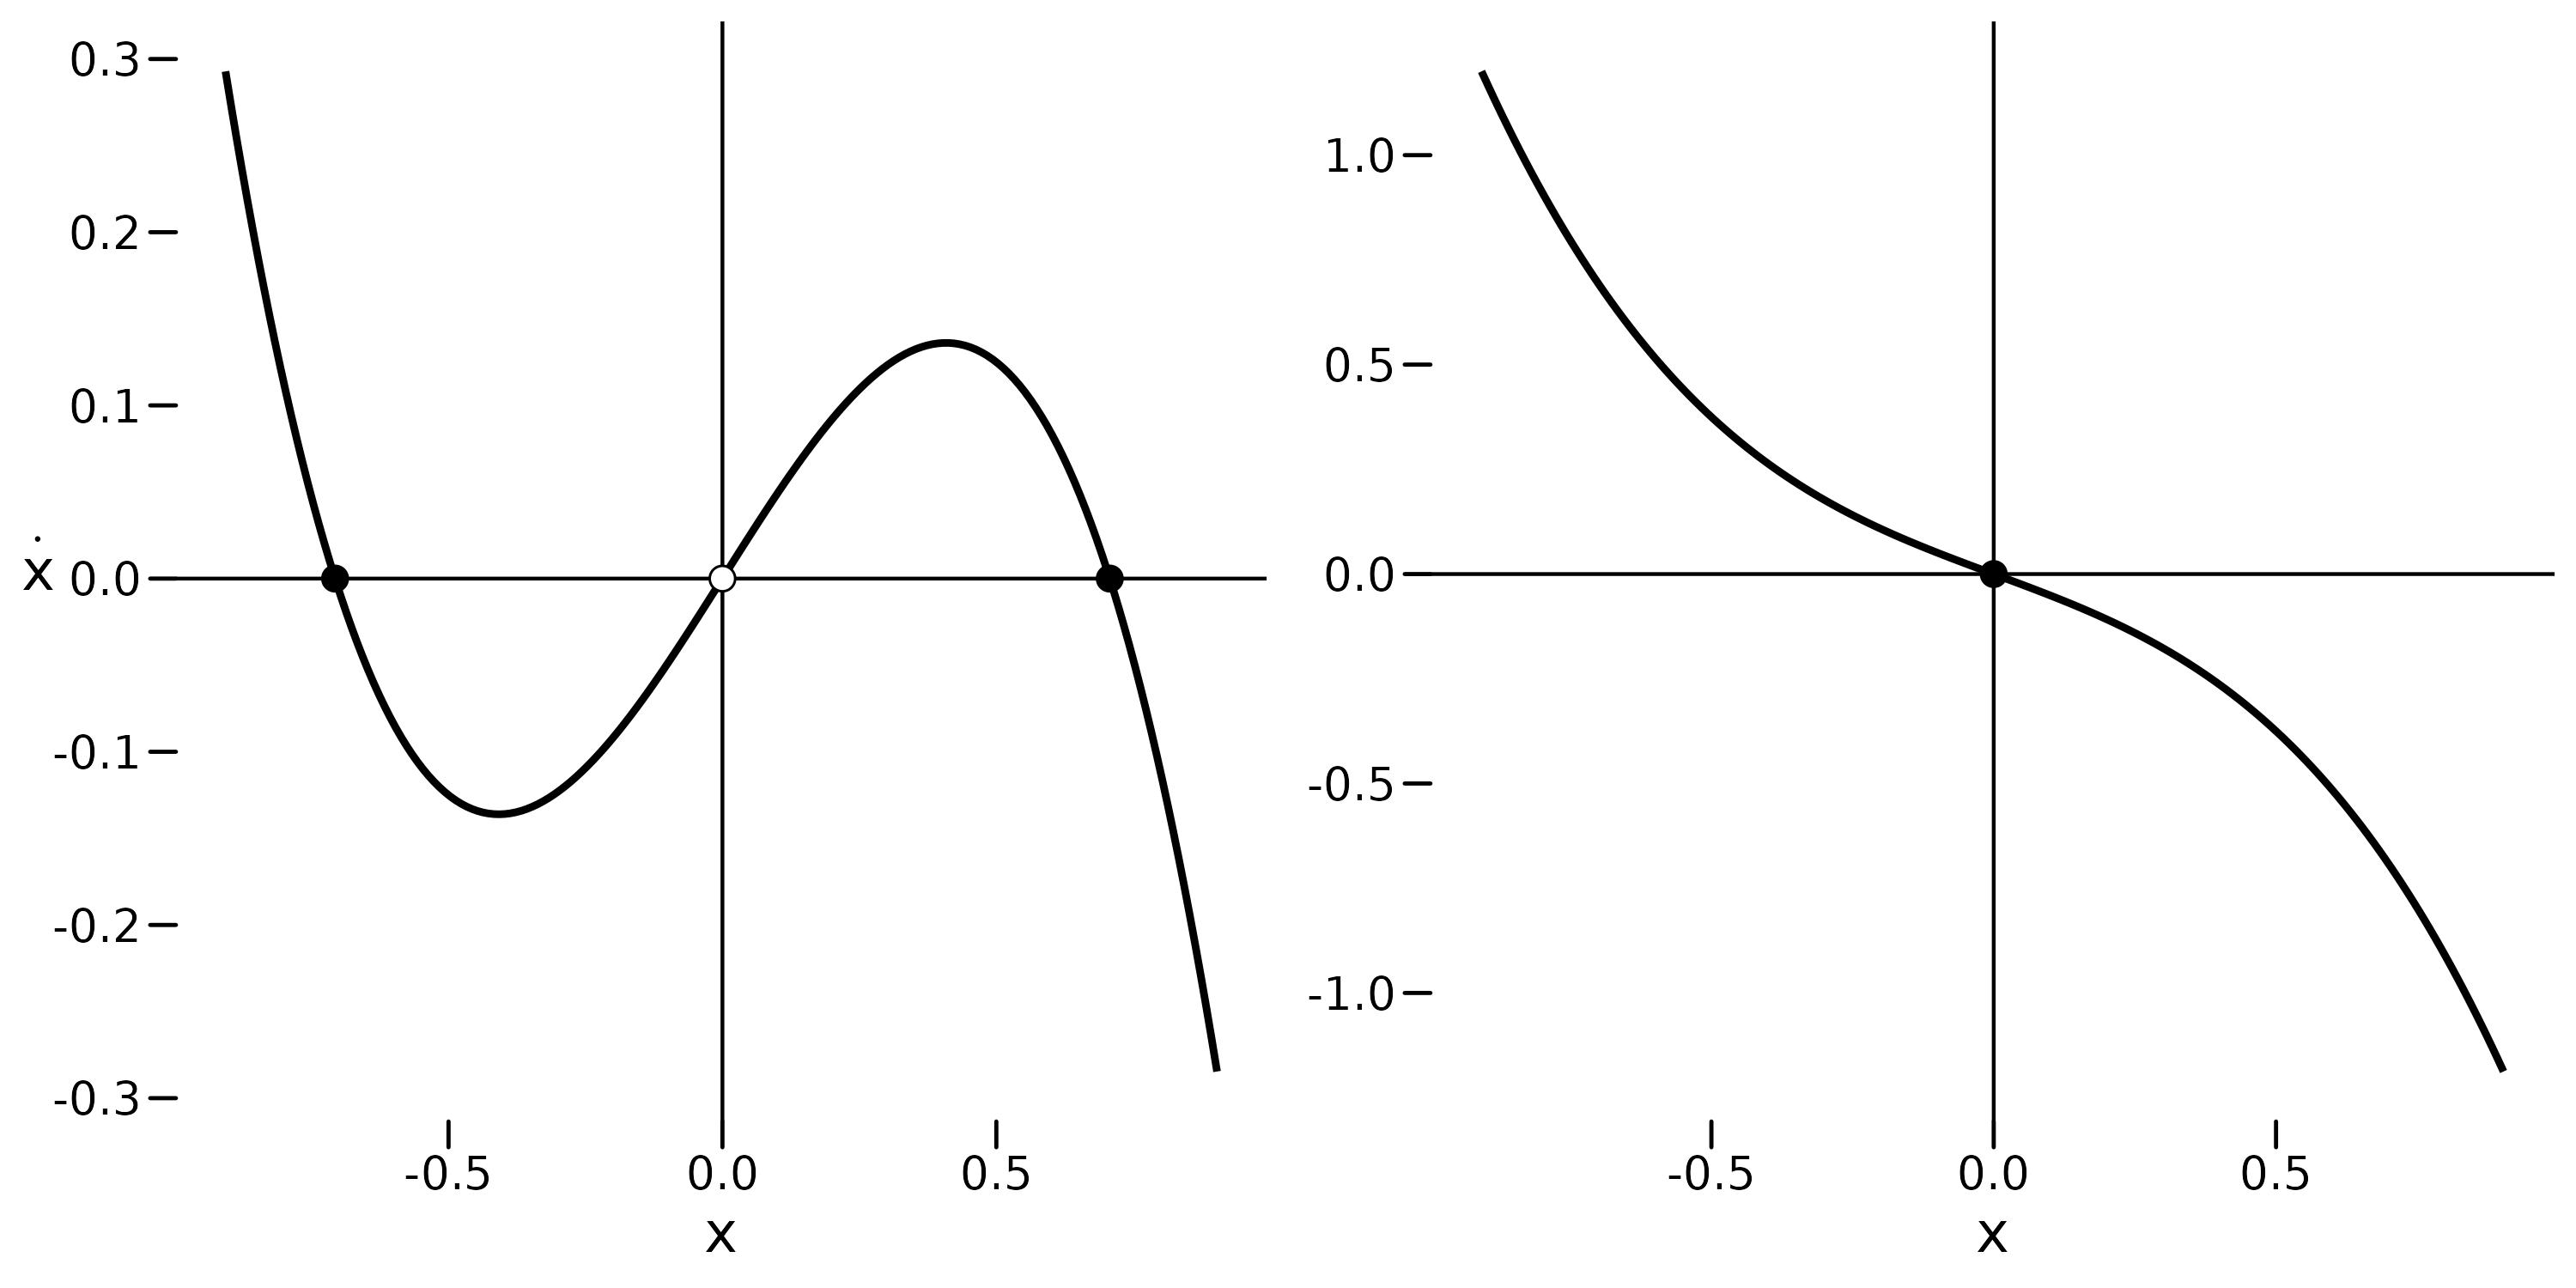
\includegraphics[scale = .125]{figures/double_well_plot_combined.jpeg}
        \caption{The value of the derivative of $X_t$ as a function of $X_t$.
        The graph on the left has $\lambda = -0.5$ and the one on the left has $\lambda = 0.5$.}
    \end{center}
\end{figure}\\
By convention the fixed points are marked by points with stable fixed points being solid points and unstable being hollow and we have fillem them in simply by looking at the graphs. When $\dot{x}_t$ i.e. $x_t'$ is below 0, the flow is to the left and otherwise. In the intercepts we have the fixed points, and by analyzing them in combination with the flow, we get the same results from the plots as we found analytically earlier. \\
The change in behaviour of the systems fixed points $\lambda$ going from negative to positive is a phenomenon that we refer to as bifurcation. What happened was that the fixed points moved closer to one another until they eventually were destroyed for $\lambda > 0$. Depending on the type of bifurcation in question this plays out differently. 
\subsubsection{Saddle-node bifurcation and Tipping Point Estimation}
In the study of dynamical systems, we refer to how changes in parameters affect the qualitative structure of the flow as bifurcations. The parameter values that results in the changes we call bifurcations points. In applications, we sometimes denote these tipping and tipping points, respectively, to get more metaphorical- and intuitive terms. \cite{Strogatz2019_gv}. Nevertheless, we only consider the so-called Saddle-node bifurcations, defined qua the normal form
\begin{align}
    X_t &= \left(\lambda \pm X_t^2\right) \mathrm{d}t \label{standardForm}
\end{align}

The fixed point of the system is always $x^* = \pm\sqrt{\abs{\lambda}}$. There is always one stable- and unstable fixed point. The stable fixed point is the negative branch of the root for the positive version of the normal form, whereas the opposite is true for the negative version. In both cases, the system has its bifurcation point at $\lambda = 0$, where the fixed point becomes half-stable. Lastly, there are no fixed-points for $\lambda>0$ in the positive version of (\ref{standardForm}) and vice versa. Now, in order to make the model more flexible we introduce the parameters, $m, A$ to shift the dynamics and scale the bifurcation point respectively. Then for values of $\lambda$ sufficiently close to the bifurcation point, $\lambda_c = 0$, any system that has the saddle-node bifurcation characteristic is approximated well by 
\begin{align}
    \mathrm{d}X_t &= \pm\left(\lambda + A\left(X_t - m\right)^2\right), 
\end{align}
with $m = \mu \pm \sqrt{\left|\frac{\lambda}{A}\right|}$ and $\mu$ is the stable fixed point of the system. \cite{Ditlevsen2023}. That is, we can be completely agnostic about the overall dynamics of the system. Yet, this naturally implies that we are completely oblivious to them as well. In our applications, the sign of the parameters, $A, \lambda$, will always be different, thus we can simplify the notation in the model to
\begin{align}
    \mathrm{d}X_t &= -\left(A\left(X_t - m\right)^2 + \lambda\right), 
\end{align}
where $m = \mu \pm \sqrt{-\frac{\lambda}{A}}$ the branch corresponds to the sign of $A$. Again, $\mu$ is the stable fixed point of the system. Now, to incorporate uncertainties into the model, we add a noise-term driven by a brownian motion
\begin{align}
    \mathrm{d}X_t &= -\left(A\left(X_t - m\right)^2 + \lambda\right) + \sigma^2(X_t, t)\mathrm{d}W_t, \label{eq:dynamicsOriginal}
\end{align}
where $\sigma^2(X_t, t)$ is a function that dictates how the noise enters the system. This is a stochastic differential equation; for a motivation of this construction see \cite[Chapter 3.1-3.2]{Srkk2019}. Finally, we model the evolution in the dynamics of the system by an extension of \cite[Equation (2)]{Ditlevsen2023}. Namely
\begin{align}
    \lambda_t = \lambda_0\left(1 - \mathds{1}\left(t>t_0\right)\frac{\left(t - t_0\right)}{\tau_c}\right)^\nu \label{eq:lambda_t}.
\end{align}
That is we use the particular form of (\ref{eq:lambda_t}) in (\ref{eq:dynamicsOriginal}). We imagine that our systems exists in some stationary state with $\lambda_t = \lambda_0$ before time $t_0$, after which a ramping starts. Apart from the stochastic part, the model is the saddle-node bifurcation \cite{Strogatz2019_gv}; we study the effects of picking different functions for $\sigma^2(X_t, t)$. More specifically, we consider functions belonging to the class of stochastic differential equations named pearson diffusions. Along with the addition of the $\nu$-parameter, this is an apparent way to extend the model with additive noise presented in \cite[equation (1)]{Ditlevsen2023}. The practical motivations for this class of diffusions will later become clear as we see that the diffusions have readily available tools that allow efficient inference.
\subsection{Inference for stochastic differential equations}
Regardless of ones exact method, inference about parameters in stochastic differential equations are often done by leveraging the markov property of Itô processes. This means that in order to estimate the parameters, it is sufficient to have the transition density or approximations thereof. Getting the transtion density involves solving the Fokker-Planck equation, which for the most part is intractable, thus one employ one or more approximation methods.\\
To this end, inference is traditionally done qua the Euler-maruyama scheme. In this thesis, we only used the estimator based on this scheme in the initial development; it is fairly easy to derive, implement and it is computationally quite efficient. Yet, the estimator is biased even for moderately large stepsizes, and quite notably so in non-linear models \cite{SplittingSchemes}. Instead, we consider two other means of estimation 
\subsubsection{The Strang likelihood}
The Strang based estimator is a method based on splitting schemes. Other similar methods exists. However, for one-step predictions of transition densities Strang is proven to be superior; compare \cite[Proposition 3.4 and 3.6]{SplittingSchemes}. For one dimensional diffusions with additive noise, splitting schemes work by splitting the process into a linear SDE and a non-linear ODE
\begin{align}
    \mathrm{d}X_t^{(1)} &= -\beta(\theta)\left(X_t^{(1)} - \mu(\theta)\right)\mathrm{d}t + \sigma \mathrm{d}W_t, &&X_t^{(1)} = x_0, \\
    \mathrm{d}X_t^{(2)} &= N\left(X_t^{(2)}\right)\mathrm{d}t, &&X_t^{(2)} = x_0, \label{ODE_Split}
\end{align}
where $N$ is some non-linear function that also might depend on the parameters. Evidently, the choice of splitting is not unique, and asymptotically any splitting is equivalent. Yet, the choice might have an impact with finite samples. Additionally, one can imagine that some splittings are numerically more well-behaved. For the most part, we use the heuristic provided in \cite[section 2.3 and 2.5]{SplittingSchemes}. That is, we find the linear SDE as the linearization around the fixed points of the drift; the ODE is then the residual of the original SDE and our linear SDE. In the one dimensional case, the solution with stepsize, $\Delta t$, to the linear SDE is given by the flow
\begin{align}
    \varphi_{\Delta t}^{(1)}(x) = \exp\left(-\beta\left(\theta\right) \Delta t\right)\left(x - \mu\left(\theta\right)\right) + \mu\left(\theta\right) + \xi_{\Delta t},
\end{align}
with $\xi_{\Delta t}\sim\mathcal{N}\left(0, \Omega_{\Delta t}\right)$. That is, the flow is gaussian with mean and variance
\begin{align}
    \mu_{\Delta t}(x; \theta) &= \exp\left(-\beta\left(\theta\right) \Delta t\right)\left(x - \mu\left(\theta\right)\right) + \mu\left(\theta\right) \label{linearSDEMean}\\
    \Omega_{\Delta t} &= \frac{\sigma^2}{2\beta}\left(1 - \exp\left(-2\beta\left(\theta\right)\Delta t\right)\right), \label{linearSDEVariance}
\end{align}
where the latter is calculated using \cite[equation (6)]{SplittingSchemes}. For our purposes the solution to (\ref{ODE_Split}) exists and is unique; with stepsize, $\Delta t$, we denote it $\varphi_{\Delta t}^{(2)}$. The conditions for this is provided in \cite[Assumption (A1) and - (A2)]{SplittingSchemes}. Then the Strang splitting scheme gives the approximation of the transition
\begin{align}
    X_{t_{i+1}}^{(S)} = \varphi_{\Delta t / 2}^{(2)}\left(\mu_{\Delta t}\left(\varphi_{\Delta t/2}^{(2)}\left(X_{t_{i}}^{(S)}\right); \theta\right) + \xi_{\Delta t} \; ; \theta \right). \label{eq:classicStrangSplitting}
\end{align}
This is a non-linear transformation of a gaussian variable; so by the density transformation theorem, the flow gives us the following negative pseudo-loglikelihood 
\begin{align}
    l^{[S]} &= -\log\left(g\left(\left(\varphi_{\Delta t / 2}^{(2)}\right)^{-1}\left(X_{t_{i+1}}\right); \mu_{\Delta t}\left(\varphi_{\Delta t/2}^{(2)}\left(X_{t_{i}}\right); \theta \right), \Omega_{\Delta t} \right) \right) \nonumber \\
    &- \log\left(\partial_x \left(\varphi_{\Delta t / 2}^{(2)}\right)^{-1} \right), \label{Strang_likelihood}
\end{align}
and we say that the $\theta$ that minimizes this expression is the Strang-based estimator. In (\ref{Strang_likelihood}) $g$ is the density of the gaussian distribution with the specified mean and variance. For the above arguments to be valud, we require additive noise in the models, which we of course get by means of the lamperti-transform. In rare instances, there exists other closes form solutions to linear stochastic differential equations than the one with additive noise. This novel splitting strategy avoids using the Lamperti-transform; although it is not central to the, we still explore the option in (\ref{meanrevertingGBMSplit1}).
\subsubsection{Approximately Optimal Martingale Estimation Equations}\label{subsubsec:approximatelyOptimalMartingaleEstimationEquation}
Other than the strang splitting, we also estimate the parameters by means of the following approximately optimal martingale estimation functions \cite[Example 1.11]{StatisticalMethodsForSDE}.
\begin{align}
    G_N^{\circ} &= \sum_{i = 1}^N 
    \left(
        \frac{\partial_\theta b\left(X_{t_{i-1}};\theta\right)}{\sigma^2\left(X_{t_{i-1}};\theta\right)}
    \right) \left(X_{t_{i}} - \mathbb{E}\left[X_{t_{i}} \middle| X_{t_{i-1}} = x\right]\right) \nonumber \\
    &+ \frac{\partial_\theta\sigma^2\left(X_{t_{i-1}}; \theta\right)}{2\sigma^4\left(X_{t_{i - 1}}; \theta\right)\Delta t}\left(\left(X_{t_{i}} - \mathbb{E}\left[X_{t_{i}} \middle| X_{t_{i-1}} = x\right]\right)^2 - \textrm{Var}\left[X_{t_{i}} \middle| X_{t_{i-1}} = x\right]\right) \label{eq:approximatelyOptimalMartingale}
\end{align}

\subsection{Numerical Optimization in \code{R}}
For each part of the process, we optimize a bit differently. However, in both cases the optimization is done with \code{stats::optim} \cite{Rlang} and our optimization methods are built as a wrapper around this function. To match the optimization done in \cite{Ditlevsen2023}, we use the Nelder-Mead algorithm in the dynamic part. In the stationary part, on the other hand, we use the BFGS-algorithm for its robustness. The wrapper is implemented such that it is possible to supply any of the likelihood functions to it. In addition, one can specify any other optimization algorithm that is implemented in \code{optim}. For the dynamic part, we also have to provide the values for $\alpha_0, \mu_0, \sigma$. We do this in the form of the estimated values for these from the stationary part of the processes. This part also dynamically chooses to estimate the $\nu$-parameter dependending on the dimension of the initial values given to the optimizer. If the dimension is two then we assume $\nu = 1$, while a dimension of three allows the optimizer estimate it. With regards to the numerical stability of the implementations we do a few things. Firstly, terms including $\exp\left(x\right) - 1$ or its additive inverse show up in many of our formulas. This is for instance the case in (\ref{linearSDEVariance}). As the arguments for the exponential function often is quite close to zero in these applications, we need to take care in order to avoid catastrophic cancellation. For this purpose, we make use of the \code{base::expm1} method in \code{R}, which calls the C-function of the same name \cite{cppreference_expm1}. Had we not done this, we would risk our program failing, because (\ref{linearSDEVariance}) would due to catastrophic cancellation evaluate to zero.
\subsection{Model diagnostics}
When we are in a simulation setting, we assess the precision of our estimation methods using the mean of the absolute relative error over a number of simulations, $M$, each with sample size, $N$. This is for the $i$th-coordinate in our parameter vector defined as
\begin{align}
    \mathrm{ARE}\left(\theta_N^{(i)}\right) = \frac{1}{M}\sum_{j = 1}^M\frac{\left|\theta_{N,j}^{(i)} - \theta_{0,j}^{(i)}\right|}{\theta_{0,j}^{(i)}}.
\end{align}
Of course, we are not able to calculate this quantity when we do not have access to the ground-truth parameters. Instead, we use uniform residuals. These require that we have a transition density, $p_\theta(x|\Delta t, x_0)$. However, in most cases we must approximate this. Nevertheless, we then also have an approximation for the conditional distribution function, $F_\theta(x|\Delta t, x_0)$, and we know $F_\theta(X_{t_{i}}|\Delta t, X_{t_{i - 1}})\sim \mathrm{Unif}(0,1)$ if $X_{t_{i}}|X_{t_{i - 1}} \sim p_\theta$. Transforming this quantity with the quantile function of the standard gaussian distribution; we may assess the fit using ordinary Q-Q plots.\\
As the approximately optimal martingale estimation functions approximate the score function, we do not have any approximation of the transition density here. Even still, we can do diagnostics, but only of the square-root process. To see how, let $X_t$ to be governed by the square-root process, then
\begin{align}
    Y_{t_{i + 1}} := \frac{4\beta}{\sigma^2\left(\exp\left(-\beta \Delta t\right) - 1\right)}X_{t_{i + 1}}
\end{align}
has transition density of a non-central $\chi^2$-distribution with $\frac{4\beta\mu}{\sigma^2}$ degrees of freedom with non-centrality parameter $Y_{t_k}\exp\left(-\beta \Delta t\right)$ \cite[Equation (5.68)]{Srkk2019}. For the other diffusions, we do not have an analagous property to exploit, and we may only assess the score function based estimators by ensuring that the estimates are consitent with methods based on the transition density; for which we use the uniform residuals.